\documentclass{beamer}
\usepackage{lmodern}
\usepackage[frenchb]{babel}
\usepackage[T1]{fontenc}
\usepackage[utf8]{inputenc}
\usepackage{graphicx}

\addtobeamertemplate{navigation symbols}{}{%
\usebeamerfont{footline}%
\usebeamercolor[fg]{footline}%
\hspace{1em}%
\insertframenumber/\inserttotalframenumber
}


\usetheme{Warsaw}

\title{Algorithmique Répartie}
\author{Jeremy Krebs - Guillaume Soulié}
\institute{Université Paris Saclay}
\date{\today}

\begin{document}

\begin{frame}
\titlepage
\end{frame}

% --------- Sommaire ---------
\begin{frame}
  \tableofcontents
\end{frame}      
% ----------------------------



\section{Introduction}

\subsection{State of the Art}
\begin{frame}
	Background and Motivations:
	\begin{itemize}
		\pause
		\item \textbf{mobile robot network} goal: achieve tasks by a team of 
		mobile robot with weak capacity. 
		\pause
		\item \textbf{Pioneering work} Suzuki, I., \& Yamashita, M. (1999). Distributed anonymous mobile robots: Formation of geometric patterns.
		\pause
		\item it studies \textbf{self-stabilizing} algorithms for anonymous and oblivious robots in uniform ring network.
	\end{itemize}
\end{frame}

\begin{frame}
	\begin{center}
		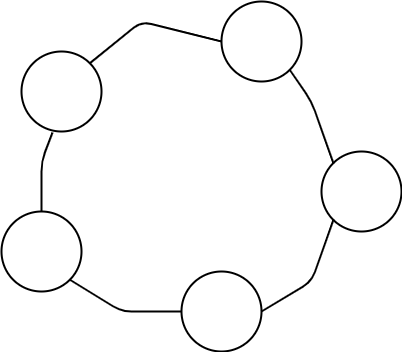
\includegraphics[width=0.7\textwidth]{images/init0.png}
	\end{center}
\end{frame}
\begin{frame}
	\begin{center}
		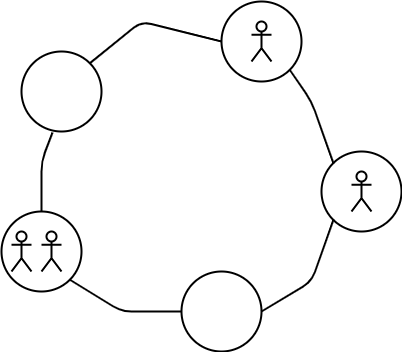
\includegraphics[width=0.7\textwidth]{images/init1.png}
	\end{center}
\end{frame}
\begin{frame}
	\begin{center}
		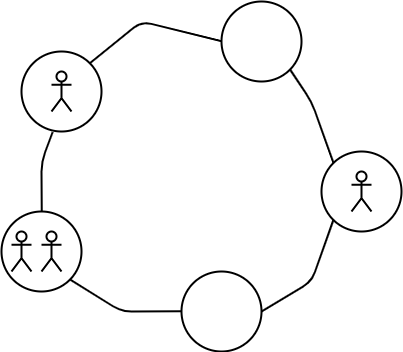
\includegraphics[width=0.7\textwidth]{images/init2.png}
	\end{center}
\end{frame}
\begin{frame}
	\begin{center}
		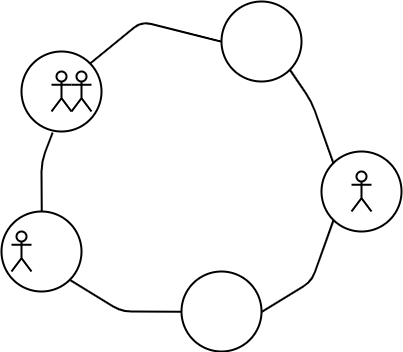
\includegraphics[width=0.7\textwidth]{images/init3.png}
	\end{center}
\end{frame}

\begin{frame}
	Each robot repeat cycles. Cycle has three phases:
	\begin{center}
		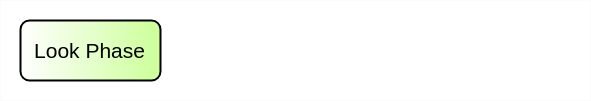
\includegraphics[width=0.9\textwidth]{images/cycle1.png}
	\end{center}
\end{frame}
\begin{frame}
	Each robot repeat cycles. Cycle has three phases:
	\begin{center}
		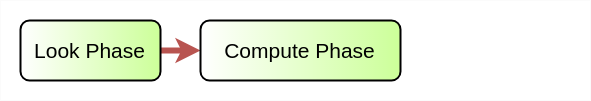
\includegraphics[width=0.9\textwidth]{images/cycle2.png}
	\end{center}
\end{frame}
\begin{frame}
	Each robot repeat cycles. Cycle has three phases:
	\begin{center}
		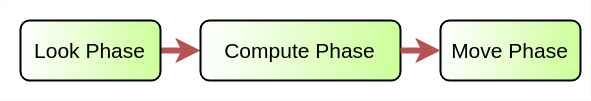
\includegraphics[width=0.9\textwidth]{images/cycle3.png}
	\end{center}
\end{frame}

\begin{frame}
	Our Contribution: investigate the difficulty of probabilistic self-stabilizing algorithms 
	using weak assumptions.
	\begin{itemize}
		\pause
		\item no such algorithms on very weak condition (ASYNC or global-weak multiplicity)
		\pause
		\item we propose three algorithms:
		\begin{description}
			\item[self-stabilizing gathering algorithm]
			\item[self-stabilizing orientation algorithm]
			\item[self-stabilizing formation algorithm]
		\end{description}  
	\end{itemize}
\end{frame}

\begin{frame}
	Related work:
	\begin{itemize}
		\pause
		\item Several work on \textbf{continuous model.} 
		\pause
		\item other work on \textbf{discrete model:}
		\begin{itemize}
			\pause
			\item deterministic / stochastic
			\pause
			\item none of them are self stabilizing
		\end{itemize}
	\end{itemize}
\end{frame}

\subsection{Hypotheses}
\begin{frame}
	There are a few hypotheses on the robots:
	\begin{itemize}
		\item<2-> Robots are identical. No distinction, same algorithm,
		\item<3-> Robots are oblivious. They have no memory of their moves,
		\item<4-> Robots cannot communicated directly.
	\end{itemize}
	
	\uncover<5->{However they can observe the positions of the other robots, and it is one of those two cases:}
	\begin{itemize}
		\item<6-> Global-Strong Multiplicity Detection
		\item<7-> Local-Strong and Global-Weak Multiplicity Detection
	\end{itemize}
\end{frame}
\begin{frame}
	The scheduler can be of two types:
	\begin{itemize}
		\item<2->[SSYNC] Semi-Synchronous - For each round, a set of robots are activated/executed at the same time.
		\item<3->[ASYNC] Asynchronous - The robots are activated/executed asynchronously
	\end{itemize}
\end{frame}

\subsection{Problems}
\begin{frame}
	\uncover<1->{
	\textbf{Gathering Problem:}
	The goal of the gathering problem is to group all the robots on the same node.}
	
	\uncover<2->{
	\textbf{Orientation Problem:}
	The goal of the set formation problem is to make the robots gather in a configuration such that:} 
	
	\begin{itemize}
		\item<3-> There is exactly one tower node
		\item<4-> There is a 1-robot block of size l
	\end{itemize}

	\uncover<5->{
	\begin{figure}[h]
   		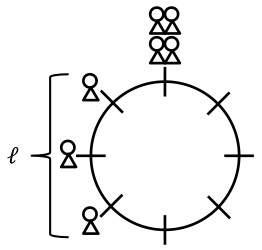
\includegraphics[width=0.3\textwidth]{images/orientation_problem.png}
	\end{figure}}
	
	\uncover<6->{
	\textbf{Set formation problem:}
	The goal of the set formation problem is to gather the robots in a specific predefined configuration.}
\end{frame}


\section{Weaker models}
\begin{frame}
	Proof of the non existence of gathering algorithm in two weak conditions:
	\begin{itemize}
		\pause
		\item ASYNC Model
		\pause
		\item SSYNC Model - global-weak \& local-strong multiplicity
	\end{itemize}
	\pause
	How to prove non existence of an algorithm ? \pause \textbf{play the scheduler}
\end{frame}
\subsection{ASYNC Model - global-strong multiplicity detection}
\begin{frame}
	(absurd) We assume that there is a algorithm $A$ which works with probability at least $p(k, n)$.  \\
	\pause
	We assume that we have a procedure $Proc(X)$ such as:
	\begin{enumerate}
		\item $Proc(X)$ activate each robot at least one
		\pause
		\item $Proc(X)$ is complete in finite time
		\pause
		\item if $P(X):=$ probability that there is no robot change during $Proc(X)$ execution,
		then $\lim_{X->\inf}{P(X)} = 1$ 
	\end{enumerate}
	\pause
	Probability that $A$ achieve gathering in $j$ cycle:
	\begin{center}
		\begin{math}
			P^* < (1-P(X_1)) + (1-P(X_2)) + ... + (1-P(X_j)) < p
		\end{math}
		$\Box$
	\end{center}
\end{frame}
\begin{frame}
	Construct $Proc(X)$:
	\begin{itemize}
		\pause
		\item one robot per node
		\pause
		\item 	$Q = +i\ (0 \leq i \leq n)$ indicates $(v_0, ..., v_{i-1})$ decides to move forward. \\
		\pause We want to achieve $Q = +n$ or $Q = -n$.
	\end{itemize}
\end{frame}

\begin{frame}
	In $proc(X)$, scheduler repeat following steps:
	\begin{itemize}
		\item if $Q = 0$: look and compute phases on robot $r$ on $v_0$:
		\begin{itemize}
			\item if $r$ want to stay => $Q:=0$
			\item elif $r$ want to move forward => $Q := 1$
			\item elif $r$ want to move backward => $Q := -1$
		\end{itemize}
		\pause
		\item if $Q = +i$: look and compute phases on robot $r$ on $v_{+i}$:
		\begin{itemize}
			\item if $r$ want to stay => $Q := +i$
			\item if $r$ want to move forward => $Q := +(i+1)$
			\item if $r$ want to move backward: move phase for $r$ and robot of $v_{+(i-1)}$
			 => $Q := +(i-1)$.	
		\end{itemize}
		\pause
		\item if $Q = -i$: ...
	\end{itemize}
	\pause
	Stop when $Q = +n$ or $Q = -n$ (or $X$ steps).
\end{frame}
\begin{frame}
	\begin{itemize}
		\item prop 1 and 2 or clearly statisfied.
		\pause
		\item for prop 3:
		\begin{itemize}
			\item $P(Q_{h+1} -> Q_h + 1) = p_1$
			\item $P(Q_{h+1} -> Q_h - 1) = p_2$
			\item $P(Q_{h+1} -> Q_h) = 1 - p_1 - p_2$
		\end{itemize}
		\pause
		This implies from any configuration $Q$, $Q = +/- n$ is achieved is less than $2n$
		step with probability $p > p_1^{2n} + p_2^{2n}$.
		\pause
		\begin{center}
			\begin{math}
				P(X) \geq 1 - (1 - p_1^{2n} - p_2^{2n})^{\frac{X}{2n}}
			\end{math} \\ 
			\pause
			\begin{math}
				\lim\limits_{X \to \inf}{P(X)} = 1
			\end{math}
		\end{center}
	\end{itemize}
\end{frame}
\subsection{SSYNC Model - global-weak / local strong multiplicity detection}

\section{Gathering Problem}
\subsection{Problem}
\begin{frame}
\textbf{Gathering problem:}

	\begin{itemize}
		\item<2-> We consider n nodes and k robots in an unoriented ring
		\item<3-> For any configuration C we not M(C) the maximum number of robots on one node
	\end{itemize}
	
	\uncover<4->{
	\begin{figure}[h]
   		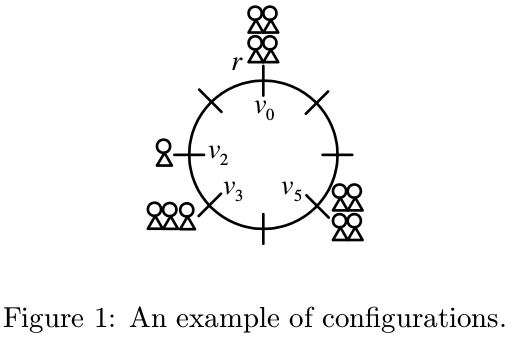
\includegraphics[width=0.3\textwidth]{images/random_configuration.png}
	\end{figure}}
\end{frame}

\subsection{Algorithm}
\begin{frame}
	Idea: 
	\begin{itemize}
		\item If there is only once M(C)-node, then the robots "know" where to go
		\item If there is multiple, the idea is to try to make them move one by one so that a tower node "wins the fight". We must find a why to elect a candidate.
		\item If there are multiple candidates, find a way to make, in expectation, exactly one of them move
		\item<2-> \textbf{Take care!} The scheduler is an enemy and will activate the robots in the worst way.
	\end{itemize}
	
\end{frame}

\begin{frame}

	Let's consider the M(C) nodes:
	\begin{itemize}
		\item[Case 1]<2-> There is only one such node: the tower can be identified by the robots and they can get closer to the tower node.
		\begin{itemize}
			\item<3-> \textbf{The scheduler is an enemy!}
			\item<3-> Less than M(C) nodes should move in the same direction! 
		\end{itemize}
	\end{itemize}

\end{frame}

\begin{frame}
	\begin{itemize}
		\item[Case 2] There are multiple such nodes:
			\begin{figure}[h]
   				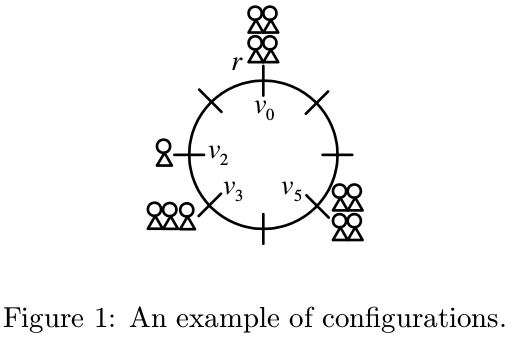
\includegraphics[width=0.2\textwidth]{images/random_configuration.png}
			\end{figure}
			\uncover<2->{Take $h_{min}$ the minimal distance between a M(C)-robot node and a neighboring robot node. Take V the set of nodes at distance $h_{min}$ of a M(C)-node and R the robots on these nodes.}
			\begin{itemize}
				\item[Cas 2.1]<3->$|R| = 1$ - This robot gets to his closer M(C)-robot node. 
				\item[Cas 2.2]<4->$|R| > 1$ - The robots move to their close M(C)-robot node with probability $\frac{1}{2|R|}$.
			\end{itemize}
	\end{itemize}
	\uncover<5->{Complexity: $O(n$ log $k)$ rounds and $O(kn)$ moves.}
\end{frame}





\section{Orientation Problem}
\begin{frame}
	Algorithm for self oriented problem:
	\begin{itemize}
		\item based on gathering algorithm
		\pause
		\item two phases algorithm
		\pause
		\item ! gathering or orientation ?
		\pause
		\item complexity: $\mathcal{O}((\log{k} + l)n)$ expected rounds 
		and $\mathcal{O}(l(k+n))$ expected moves
	\end{itemize}
\end{frame}

\begin{frame} 
	Phase 1:
	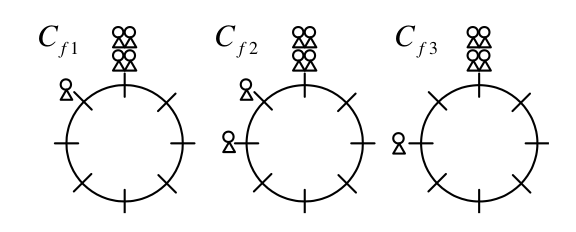
\includegraphics[width=0.9\textwidth]{images/orient1.png}
	\pause
	Reaches a configuration $C_{f1}$ (if $l = 1$) or in $C_{f2}$ (if $l \geq 2$)
	 in $\mathcal{O}(n \log{k})$ expected rounds and $\mathcal{O}(kn)$ expected moves.
\end{frame}

\begin{frame}
	Phase 2:
	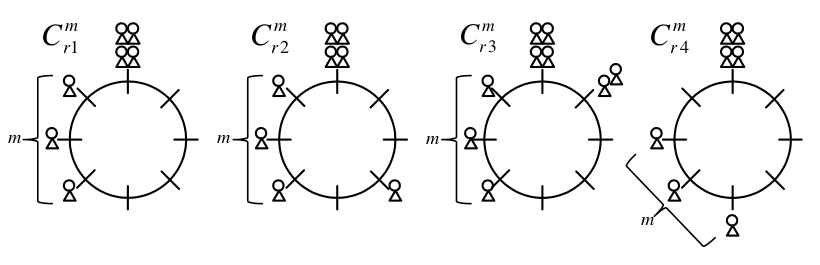
\includegraphics[width=0.9\textwidth]{images/orient2.png}
	\pause
	Reaches a configuration in $C_0$ in $\mathcal{O}(ln)$ expected rounds and $\mathcal{0}(l(k+n))$ expected moves.
\end{frame}

\section{Set Formation Problem}
\begin{frame}
	We can now apply the two previous algorithms to solve the \textbf{set formation problem}.
\end{frame}

\begin{frame}
	\begin{itemize}
		\item<1-> Solve the orientation algorithm for $l = |SET| - 1$,
		\item<2-> Now that the ring is oriented, move the robots one by one
	\end{itemize}
	\uncover<3->{
		\begin{figure}[h]
   			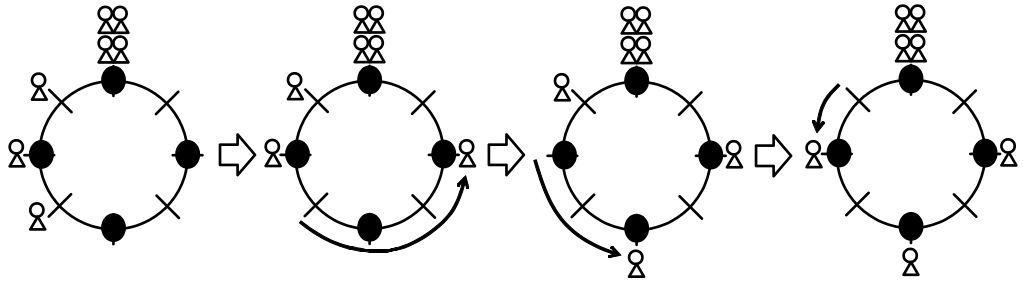
\includegraphics[width=0.9\textwidth]{images/set_formation.png}
		\end{figure}}
	
	\uncover<4->{Complexity: $O(($log $k + |SET|)n)$ rounds and $O(kn)$ moves.}
\end{frame}


\section{Conclusion}
\begin{frame}
	\textbf{Conclusion:}
	\begin{itemize}
		\item<2-> Our strong assumptions on the system are mandatory
		\item<3-> Solving the gathering and orientation issues is very important and leads to tons of other problems solved
	\end{itemize}
	
	\uncover<4->{\textbf{In order to go further we could:}}
	\begin{itemize}
		\item<5-> Find the problems we can solve with weaker hypotheses,
		\item<6-> Work with a weaker scheduler, like an oblivious one,
		\item<7-> Work with a more complex graph than a ring.
	\end{itemize}
	
\end{frame}
\end{document}
